\chapter{ Технологический раздел}
\label{cha:technological}

    В данном разделе будут выбраны средства реализации ПО и представлен листинг кода. 

    \section{Средства реализации}
        В данной работе используется язык программирования python \cite{python}, так как
        он позволяет написать программу в относительно малый срок.
        В качестве среды разработки использовалась Visual Studio Code \cite{visual-studio-code}.

        Для замера процессорного времени была использована функция process\_time \cite{process_time} модуля time.
        Она возвращает значение в долях секунды суммы системного и пользовательского процессорного времени текущего процесса и 
        не включает время, прошедшее во время сна.

    \section{Листинг программы}
        Ниже представлены листинги кода алгоритмов сортировки:
        \begin{enumerate}
            \item пузырьком с флагом (листинг \ref{lst:bubble});
            \item вставками (листинг \ref{lst:insertion});
            \item выбором (листинг \ref{lst:selection}).
        \end{enumerate}
        
        \begin{lstlisting}[language=python, label=lst:bubble, caption=Реализация алгоритма сортировки пузырьком с флагом]
def bubble_sort(mass, cmp = lambda a, b: a - b):
    len_mass= len(mass)
    for i in range(len_mass, 0, -1):
        need = False
        for j in range(1, i):
            if cmp(mass[j-1], mass[j]) > 0:
                mass[j-1], mass[j] = mass[j], mass[j-1]
                need = True
        if not need: break
    return mass
        \end{lstlisting}

        \begin{lstlisting}[language=python, label=lst:insertion, caption=Реализация алгоритма сортировки вставками]
def insertion_sort(mass, cmp = lambda a, b: a - b):
    len_mass = len(mass)
    for i in range(1, len_mass):
        v = mass[i]
        j = i
        while cmp(mass[j-1], v) > 0 and j > 0:
            mass[j] = mass[j-1]
            j -= 1
        mass[j] = v
    return mass
        \end{lstlisting}

        \begin{lstlisting}[language=python, label=lst:selection, caption=Реализация алгоритма сортировки выбором]
def selection_sort(mass, cmp = lambda a, b: a - b):
    len_mass = len(mass)
    for i in range(len_mass):
        min_i = i
        for j in range(i+1, len_mass):
            if cmp(mass[j], mass[min_i]) < 0:
                min_i = j
        mass[min_i], mass[i] = mass[i], mass[min_i]
    return mass
        \end{lstlisting}
    
        
    \section{Тестирование}
        В таблице \ref{table:testing} отображён возможный набор тестов
        для тестирования методом чёрного ящика, результаты которого, 
        представленные на рисунке \ref{png:testing:result}, подтверждают
        прохождение программы перечисленных тестов.

        \begin{table}[]
            \caption{Тесты для проверки корректности программы}

            \centering
            \begin{tabular}{|c|c|c|}
                \hline
                Массив                      & Ожидаемый результат           \\ \hline
                  [ ]                       &        [ ]                    \\ \hline
                  [1]                       &        [1]                    \\ \hline
                [1, 2, 3]                   &     [1, 2, 3]                 \\ \hline
                [3, 2, 1]                   &     [1, 2, 3]                 \\ \hline
                [1, 212, -5, 1, 64, -75]    &     [-75, -5, 1, 1, 64, 212]  \\ \hline
                \end{tabular}
            \label{table:testing}
        \end{table}
        
        \begin{figure}[h!]
            \centering
            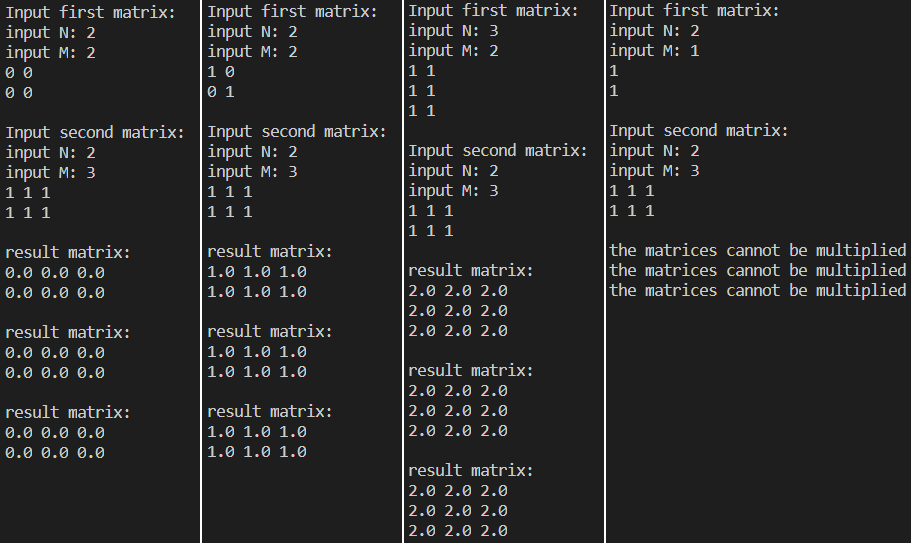
\includegraphics[scale=0.9]{testing.png}
            \caption{Результаты тестирования алгоритмов.}
            \label{png:testing:result}
        \end{figure}
\newpage